\subsection{Documentation}

Design structure includes 5 main components:
\begin{itemize}
  \item home page,
  \item forgotten password,
  \item user registration,
  \item user page,
  \item admin page.
\end{itemize}
Homepage would be something simple that users and admins have in common. When admin wants to login, login section would check if user signing in is actual user or admin. With that information, the correct page would be shown.
\begin{figure}[H]
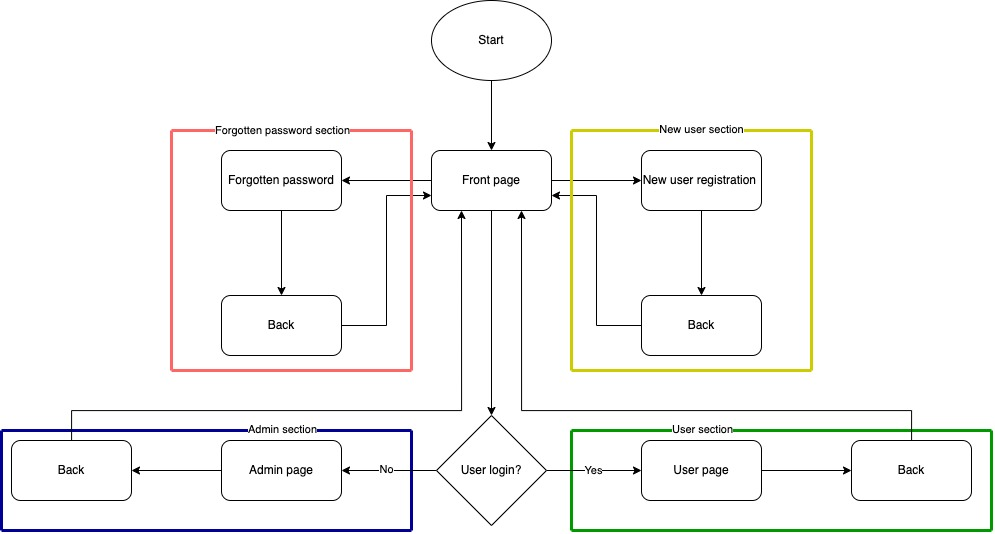
\includegraphics[scale=0.41]{img/UI-UI-simple.jpeg}
\centering
\caption{Diagram representing simple structure}
\end{figure}

Forgotten password is for users and admins to reset their passwords. Upon opening the page, user can reset the password (with inserting correct information) and be redirected to homepage. If user declines to to so, they can navigate back.
\begin{figure}[H]
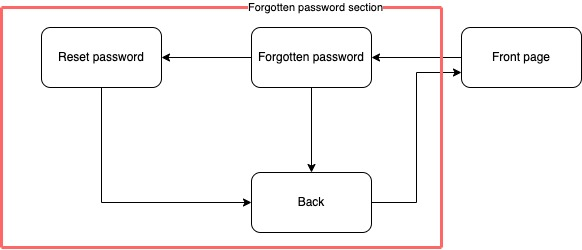
\includegraphics[scale=0.7]{img/UI-UI-forgotten-password.jpeg}
\centering
\caption{Diagram representing forgotten password}
\end{figure}

New user creation is for users to sign up for the service. On the site, user needs to fill the form in order to sign up. Once done, they are redirected to home page. If user declines to to so, they can navigate back.
\begin{figure}[H]
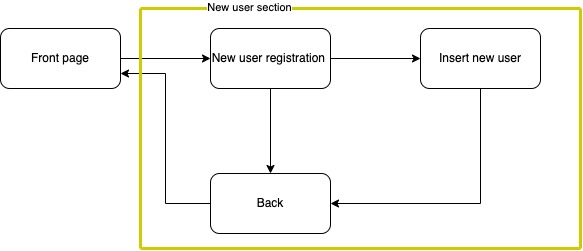
\includegraphics[scale=0.7]{img/UI-UI-new-user.jpeg}
\centering
\caption{Diagram representing new user registration}
\end{figure}

On user login, user can see how many devices he/she has per section. From there they can select section to see all devices in there. Once all devices from sections are shown, they can perform CRUD operations by adding new device, listing existing devices, adding new devices and removing existing devices.
\begin{figure}[H]
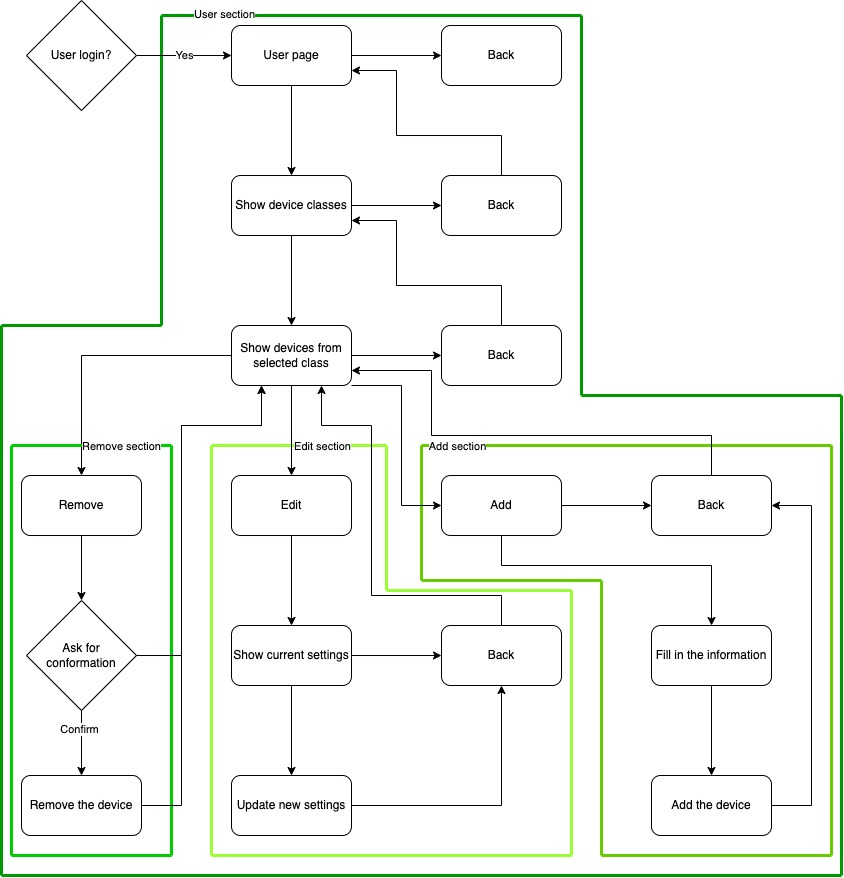
\includegraphics[scale=0.5]{img/UI-UI-users-section.jpeg}
\centering
\caption{Diagram representing user view}
\end{figure}

If user logging in is admin, he/she will be redirected to this section. In here, admin can select "show users" or "show devices" section. In case admin wants to edit user settings (promote user to admin), option is there under "show users". Another thing they can see is analysis of users (for example, usual logins). If they select "show devices", where admin can edit existing device types. Admin can also add new supported devices in "add device" section. Under device analytic, admin can see how devices are performing.
\begin{figure}[H]
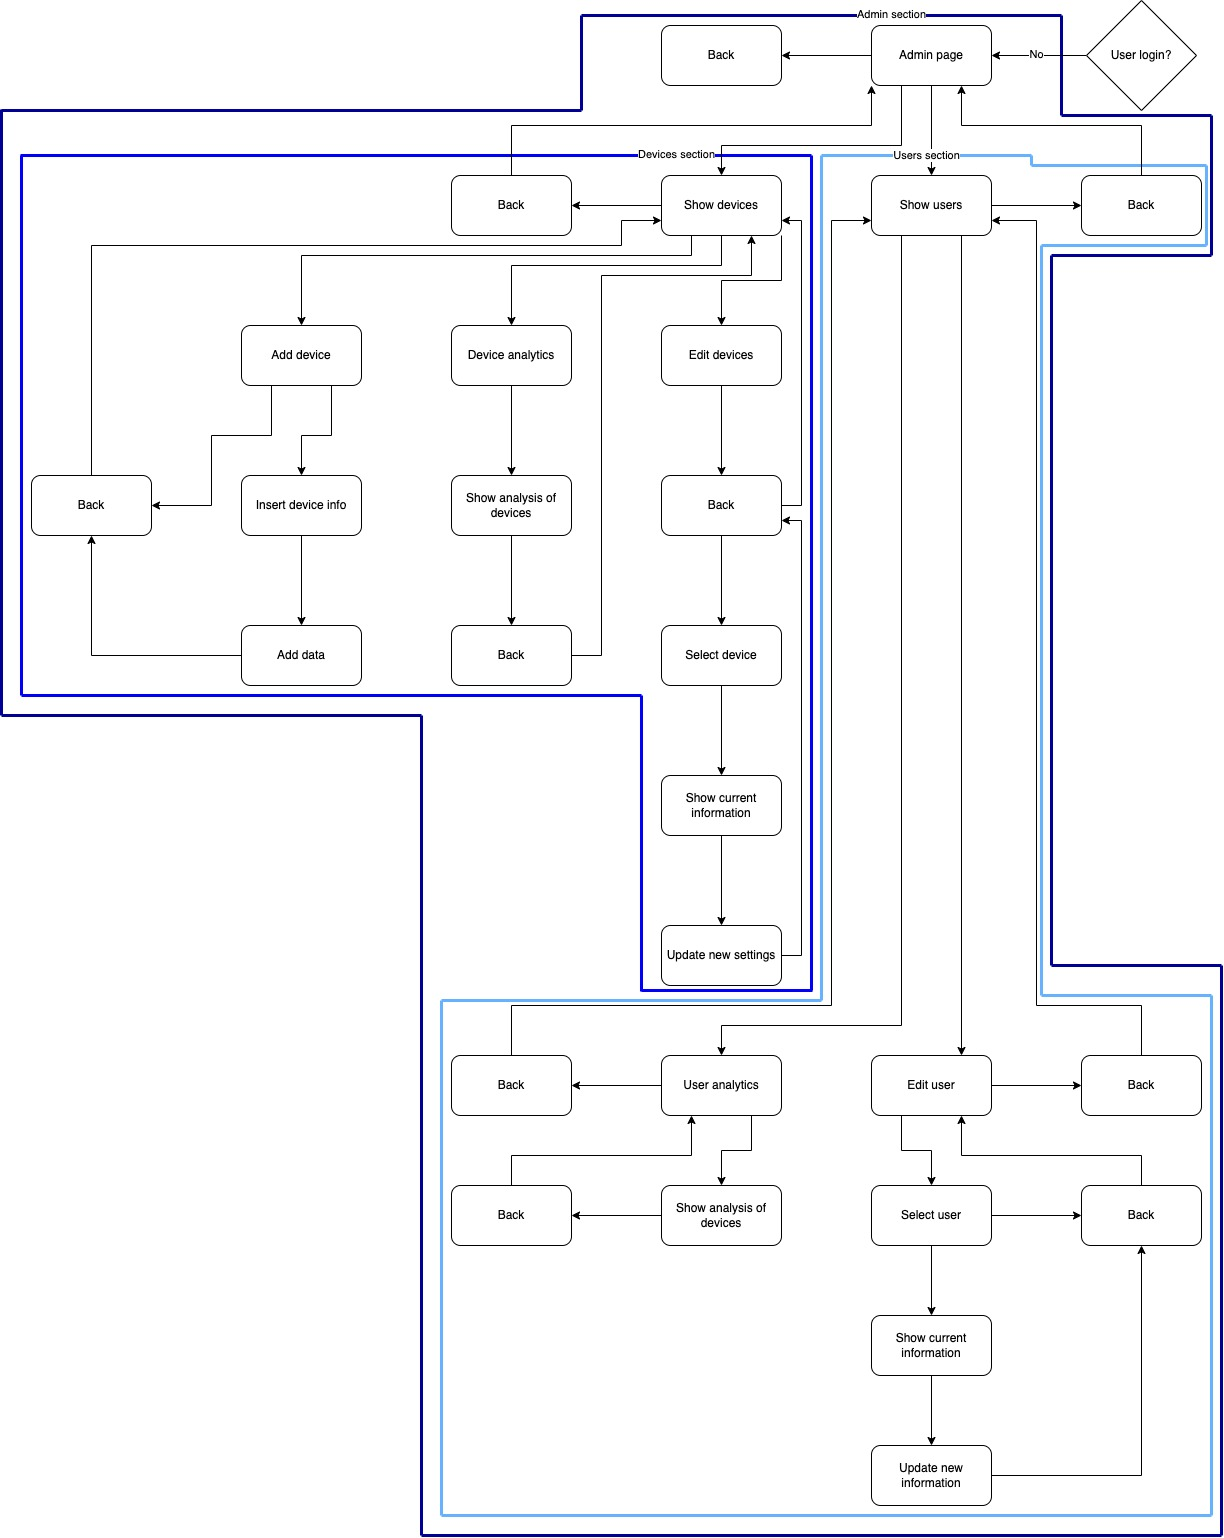
\includegraphics[scale=0.35]{img/UI-UI-admin-section.jpeg}
\centering
\caption{Diagram representing admin view}
\end{figure}

This is the same figure as on top but with all the sections expended.
\begin{figure}[H]
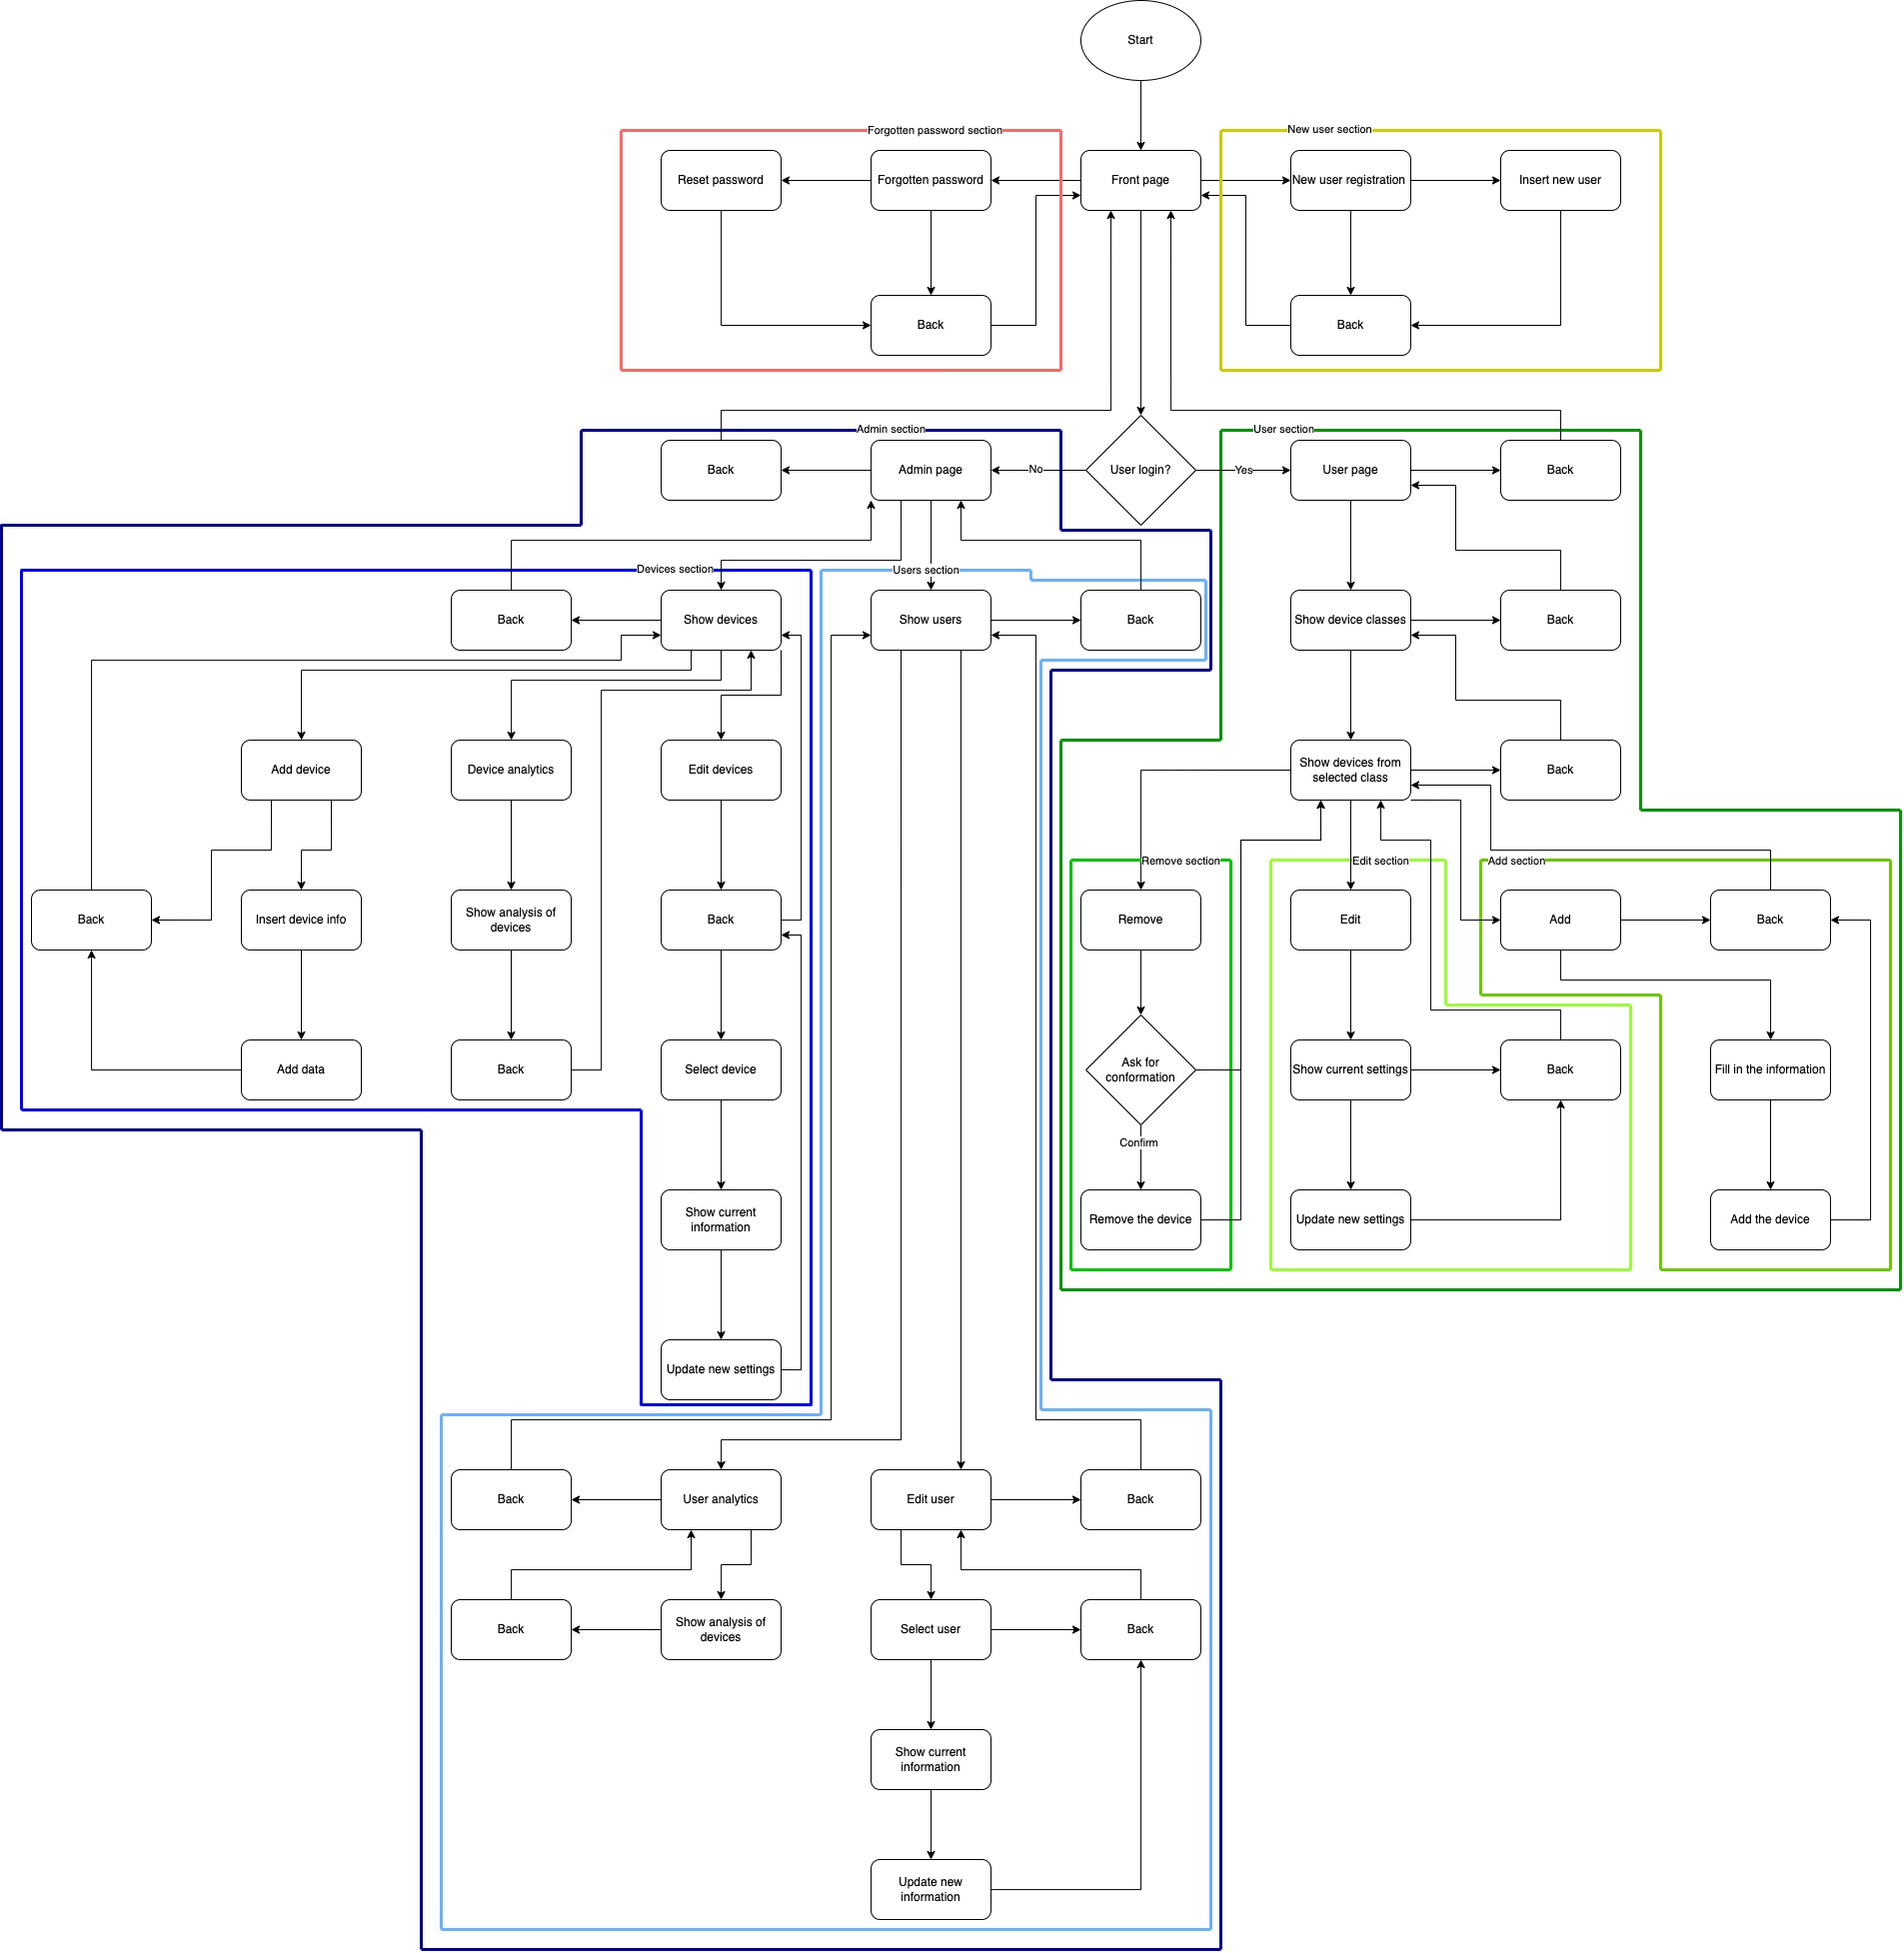
\includegraphics[scale=0.225]{img/UI-diagram.jpeg}
\centering
\caption{Detailed diagram of whole web application}
\end{figure}

